\documentclass[12pt]{beamer}
\usetheme{Rochester}
\usepackage[utf8]{inputenc}
\usepackage{amsmath}
\usepackage{amsfonts}
\usepackage{amssymb}
\usepackage{amsthm}
\usepackage{graphicx}
\usepackage{cite}
\usepackage{tikz}
\usetikzlibrary{arrows,shapes,automata,petri}
\newtheorem{myDef}{Definition}

\author{Josiah Hanna, David Tamez, and Xiaorong Zhu}
\title{Generating Petri Nets With Evolutionary Algorithms}
\institute{The University of Texas at Austin}
\date{December 3rd, 2014}
\begin{document}

\begin{frame}
\titlepage
\end{frame}

\begin{frame}{Petri Net Overview}
Petri nets are mathematical models for distributed systems.
\begin{myDef}
A Petri Net is defined as a tuple $(P,T,F,M,W)$ where $P$ is a set of place nodes, $T$ is a set of transition nodes, $F$ is a set of arcs in either $P \times T$ or $T \times P$, $M: P \rightarrow Z$ is an initial marking, and $W: F \rightarrow Z$ is an arc weight function.
\end{myDef}
\begin{figure}
\includegraphics[scale=0.25]{petri_net.png}
\caption[]{An example Petri network \label{exampleNet}}
\end{figure}
\end{frame}

\begin{frame}{Petri Net Applications and Disadvantages}
Applications
\begin{itemize}
\item Higher level robot control
\item Data analysis
\item Simulation
\item Showing correctness of a system
\end{itemize}
Disadvantages
\begin{itemize}
\item Must be hand coded which is hard for complex tasks
\end{itemize}
\vspace{5ex}
\end{frame}
\begin{frame}{Petri Net Applications and Disadvantages}
Applications
\begin{itemize}
\item Higher level robot control
\item Data analysis
\item Simulation
\item Showing correctness of a system
\end{itemize}
Disadvantages
\begin{itemize}
\item Must be hand coded which is hard for complex tasks
\end{itemize}

\bigskip

\centering{\Large{Use evolutionary algorithm to evolve them!}}
\end{frame}

%%%%%%%%%%%%%% SAME SLIDE %%%%%%%%%%%%%%%%%%%%%5
\begin{frame}{Proposed Solution}
We propose that the Neuroevolution of Augmenting Topologies (NEAT) could be used to evolve Petri Nets.
\begin{itemize}
\item NEAT evolves topologies and weights of neural networks.
\item NEAT allows complex structures to evolve through speciation.
\item We modify the NEAT genome and mutation operators
\end{itemize}
\vspace{4ex}

\end{frame}
\begin{frame}{Proposed Solution}
We propose that the Neuroevolution of Augmenting Topologies (NEAT) could be used to evolve Petri Nets.
\begin{itemize}
\item NEAT evolves topologies and weights of neural networks.
\item NEAT allows complex structures to evolve through speciation.
\item We modify the NEAT genome and mutation operators
\end{itemize}
\bigskip
NEAT becomes PetriNEAT!
\end{frame}

%%%%%%%%%% END SLIDE %%%%%%%%%%%%%%%55

\begin{frame}{Genome}
Node Genes
\begin{table}
\centering
\begin{tabular}{|c|}
\hline
Node Gene\\ \hline
I.D. \\
Type \\
Initial Tokens \\
Action I.D. \\
\hline
\end{tabular}
\end{table}

Link Gene
\begin{table}
\centering
\begin{tabular}{|c|}
\hline
Arc Gene\\ \hline
Node Place \\
Node Transition \\
Weight \\
\hline
\end{tabular}
\end{table}

\end{frame}

\begin{frame}{Genetic Operators}

We use the following mutation operators in evolving our network:
\begin{itemize}
\item mutate add node
\item mutate add link
\item mutate node
\item mutate link
\end{itemize}


\end{frame}

\begin{frame}{Adding Nodes}
\begin{columns}[]
  \begin{column}{2in}
  \begin{figure}
    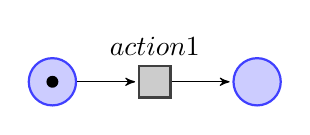
\begin{tikzpicture}[node distance=1.3cm,>=stealth',bend angle=45,auto]
  \tikzstyle{place}=[circle,thick,draw=blue!75,fill=blue!20,minimum size=6mm]
  \tikzstyle{transition}=[rectangle,thick,draw=black!75,
              fill=black!20,minimum size=4mm]
    \node [place,tokens=1] (p1){};
    \node [transition] (t1) [right of=p1, label=above:$action1$] {}  edge [pre] (p1);
    \node [place] (p2)  [right of=t1] {} edge [pre] (t1);
\end{tikzpicture}
\caption{Adding connectivity}
\end{figure}

\begin{figure}
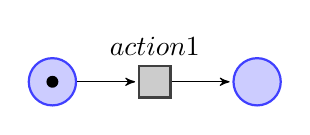
\begin{tikzpicture}[node distance=1.3cm,>=stealth',bend angle=45,auto]
  \tikzstyle{place}=[circle,thick,draw=blue!75,fill=blue!20,minimum size=6mm]
  \tikzstyle{transition}=[rectangle,thick,draw=black!75,
              fill=black!20,minimum size=4mm]
    \node [place,tokens=1] (p1){};
    \node [transition] (t1) [right of=p1, label=above:$action1$] {}  edge [pre] (p1);
    \node [place] (p2)  [right of=t1] {} edge [pre] (t1);
\end{tikzpicture}
\caption{Grow the network}
\end{figure}
  \end{column}
  \begin{column}{2in}
  \begin{figure}
    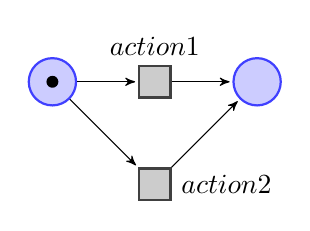
\begin{tikzpicture}[node distance=1.3cm,>=stealth',bend angle=45,auto]
  \tikzstyle{place}=[circle,thick,draw=blue!75,fill=blue!20,minimum size=6mm]
  \tikzstyle{transition}=[rectangle,thick,draw=black!75,
        fill=black!20,minimum size=4mm]
    \node [place,tokens=1] (p1){};
    \node [transition] (t1) [right of=p1, label=above:$action1$] {}  edge [pre] (p1);
    \node [place] (p2)  [right of=t1] {} edge [pre] (t1);
    \node [transition] (p3) [below of=t1, label=right:$action2$] {} edge [pre] (p1) edge [post] (p2);
\end{tikzpicture}
\end{figure}

 \begin{figure}
    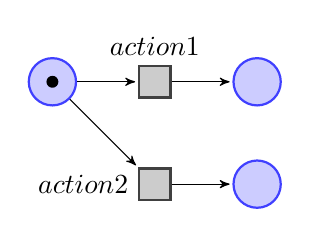
\begin{tikzpicture}[node distance=1.3cm,>=stealth',bend angle=45,auto]
  \tikzstyle{place}=[circle,thick,draw=blue!75,fill=blue!20,minimum size=6mm]
  \tikzstyle{transition}=[rectangle,thick,draw=black!75,
        fill=black!20,minimum size=4mm]
    \node [place,tokens=1] (p1){};
    \node [transition] (t1) [right of=p1, label=above:$action1$] {}  edge [pre] (p1);
    \node [place] (p2)  [right of=t1] {} edge [pre] (t1);
	\node [place] (p4) [below of=p2] {};    
    \node [transition] (p3) [below of=t1, label=left:$action2$] {} edge [pre] (p1) edge [post] (p4);
    
\end{tikzpicture}
\end{figure}
  \end{column}
\end{columns}
\end{frame}

\begin{frame}{Target Task}
We evolve Petri net solutions for a robot moving towards a goal in a grid world.
\begin{figure}
\includegraphics[trim = 80mm 80mm 20mm 70mm, clip, width = 2.4in, height = 1.6in]{robot_sim.png}
\end{figure}
We define the fitness of a potential solution to be:
$$fitness = \frac{2^{goalReached}}{1.0 + finalDistanceFromGoal + actionsTaken}$$
\end{frame}

\begin{frame}{Results}

Conclusion: It is possible to evolve Petri nets
\begin{itemize}
\item Petri net weights, markings, and structure can adapt to improve network fitness.
\item Networks evolved through mutation can solve a given task.
\item Simple building blocks can create compound actions.
\end{itemize}
\end{frame}

\begin{frame}{Resulting Structure}
\begin{columns}[]
  \begin{column}{2in}
  \begin{figure}
\includegraphics[scale=0.3]{PetriNet_1_1}

\end{figure}
\vspace{-5ex}
\begin{figure}
\includegraphics[scale=0.3,width=2in]{PetriNet_1_2}

\end{figure}
  \end{column}
  \begin{column}{2in}
  \begin{figure}
\includegraphics[scale=0.3]{PetriNet_1_3}
\vspace{-5ex}
\end{figure}
 \begin{figure}
\includegraphics[scale=0.3, width=2in]{PetriNet_1_4}

\end{figure}
  \end{column}
\end{columns}
\end{frame}

\begin{frame}{Resulting Structure}
\begin{columns}
\begin{column}{2in}
\begin{figure}
\includegraphics[scale=0.3]{PetriNet_2_1}
\end{figure}
\end{column}
\begin{column}{2in}
\includegraphics[scale=0.3]{PetriNet_2_2}
\end{column}

\end{columns}
\end{frame}

\begin{frame}{Future Work}
The next steps in exploring Petri net evolution are:
\begin{enumerate}
\item Add cross over operations to the evolutionary algorithm.
\item Explore different mutation operators.
\item Generate more complex types of Petri networks.
\item Increase the complexity of our target task.
\item Add methods to combine Petri nets into hierarchies.
\item Use reachability graph to simplify network.
\end{enumerate}

\end{frame}

\begin{frame}{References}
\bibliographystyle{plain}
\bibliography{project}
\nocite{PNP}
\nocite{stanley:gecco02a}
\end{frame}

\end{document}